%
% Frontmatter - Introducci�n. Los miembros del tribunal que juzgan los PFC's tienen muchas m�s memorias que leer, por lo que
%	agradecer�n cualquier detalle que permita facilitarles la vida. En este sentido, realizar una peque�a introducci�n,
%	comentar la organizaci�n y estructura de la memoria y resumir brevemente cada cap�tulo puede ser una buena pr�ctica
%	que permita al lector centrarse f�cilmente en la parte que m�s le interesa.
%

\chapter[Introduction]{
	Introduction
}

Computer Graphics is the discipline that deals with creating, managing, analyzing and visualizing graphics using a computer, and it is closely linked to other disciplines such as Image Processing, Computer Vision or Machine Learning, among others. Advances in computer graphics have had an impact on several media types such as, for example, the movies and video games industry, civil engineering, medicine, etc.

In computer graphics, \emph{rendering} is the process of generating a 2D image to be shown in a display. This process takes usually a virtual scene of 3D objects as input, containing data like geometry, lighting, cameras, etc.
Typically, polygonal modeling has been the approach followed for modeling objects in the scene, approximating their surfaces using polygons. Point-based graphics focuses on points as the fundamental representation of the surfaces instead of polygons (see \figurename~\ref{poly_comp}).

\begin{figure}
	\centering
	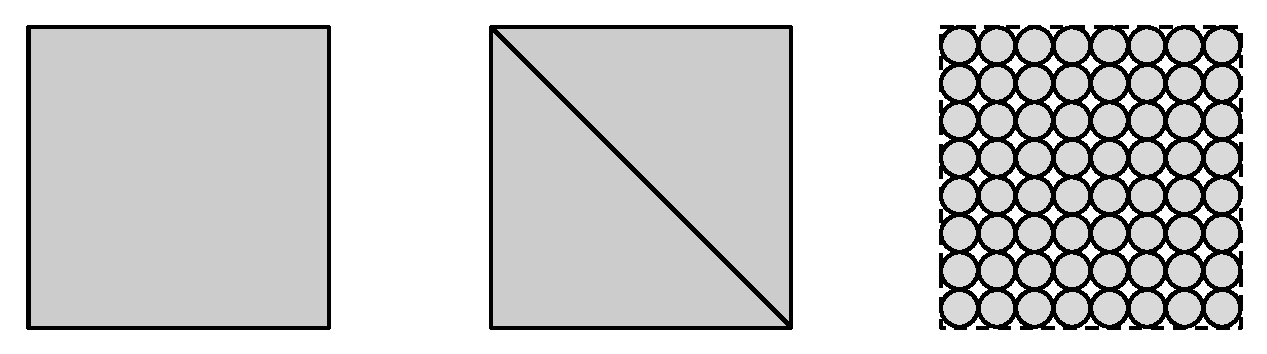
\includegraphics[scale=0.6]{figures/pol_comp.pdf}
	\caption[Modeling types comparison]{
		From left to right; mathematical representation of a plane, representation using two polygons (triangles) and a point-based representation.
	}
	\label{poly_comp}
\end{figure}

Nowadays, acquisition technologies such as LIDAR (Laser Imaging
Detection and Ranging) allow us to obtain high-precision
georeferenced 3D scans of the real world in an easy and fast way.
These systems use ultraviolet, visible or near infrared light to image objects. It can target a wide range of materials and even single molecules. A narrow laser beam can map features with very high precision.
The evolution of this kind of technologies is having a tremendous
impact in multiple fields in the engineering, and bringing back the
camp-work to the office has become a standard practice.
This presents clear advantages compared to the classical work-flow in
disciplines like topography, that usually need to come back on the
ground each time a new measurement is required. A couple of images
obtained from a LIDAR scanner are shown in
\figurename~\ref{lidarexamples}.

\begin{figure}
  \centering
  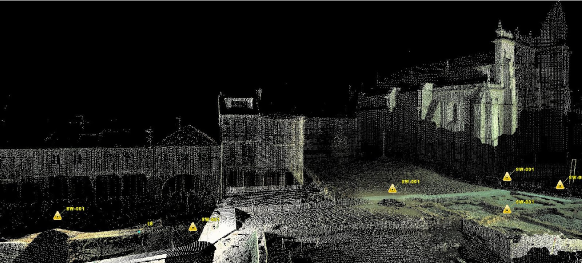
\includegraphics[width=0.475\textwidth]{figures/campillo1.png} \quad
  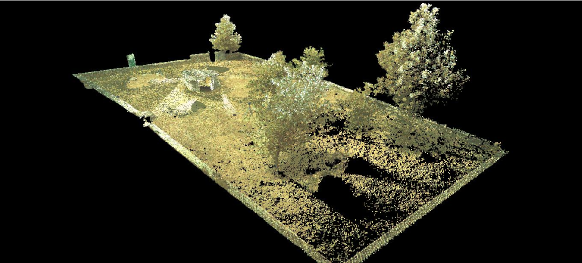
\includegraphics[width=0.475\textwidth]{figures/parcela.png}
  \caption{Examples of LIDAR scanning.}\label{lidarexamples}
\end{figure}

These scanning devices generate data-sets with an enormous number of
samples, with 3D coordinates and additional data such as color,
reflectivity and so on. These point clouds, as they are usually
named, are formed by hundreds or thousands of points, resulting in
Giga or even tera-bytes of information.
Using point based representations, the polygonal approximation step
can be skipped and the massive amount of captured data is directly
used. However, managing these huge data-sets, either for applying some kind of data
analysis or for visualization, is a computational challenge and an
open and state-of-the-art problem. This project deals with this question.

This chapter introduces the motivation behind the project and the
objectives we try to achieve. It shows the structure of this document
as well.

\section[Motivation and context]{
	Project motivation and context
}

PCM is a software library developed in the University of A Coru�a for the management of huge point datasets obtained by LIDAR in commodity hardware systems. It was started as a MSc Final Project~\cite{Jaspe12} (system structure and basic capabilities) in the Faculty of Computer Science and then continued in a BSc Final Project~\cite{Jaspe13} (improved render and other minor additions).

PCM is based on a multi-resolution structure and includes basic memory hierarchy management, making it possible to transfer the point cloud data between secondary memory (HDD) and video memory in the graphics card. Originally, PCM includes a very basic visualizer, quite simple and limited but that has the potential to become the seed for a more advanced point cloud software tool that will allow the user to access all of these features in real-time.

Although PCM was designed to deal with arbitrary size datasets, it is far from being a mature software and has some problems managing point clouds in the order of billion points. Because of the massive nature of these datasets, achieving real-time manipulation of them is a complex task. It will require the improvement of PCM, with a complete profiling and performance analysis and a careful refactoring. Having a system that is able to manage such a huge amount of data, will let the user take advantage of the full potential of cutting-edge 3D capture devices.
Of course, the library should exploit the full potential of both modern CPUs and GPUs, automatically using parallel processing to reduce the computation time as much as possible.
Furthermore, although PCM sketches a framework for applying data
analysis on the point clouds, this part was barely crafted at
all. Other constraints of the original proposal are also addressed in
this work, such as adding read/write operations to allow the
modification of the datasets, the possibility of working with multiple
point clouds, etc.

In this project, a complete user-oriented software suite for the visualization, management, analysis and manipulation of massive 3D point clouds will be developed from the original PCM proposal. ToView is the name chosen for this software package. It is a multi-platform (GNU/Linux, Windows and MacOS) free software project and makes use of open source software exclusively. For these reasons the user interface is based on the cross-platform application framework QT, that has native implementations and tools for all the aforementioned platforms. The resulting QT application will let the user access all of the functionality including an advanced and complete 3D visualizer.

\section[Objectives]{
	Project objectives
}

The aim of this project is the design and implementation of a point-based multi-platform software tool for the interactive visualization, management, analysis and manipulation of massive 3D point clouds. 

The application will offer the user the necessary tools to work effectively with this type of datasets, including a 3D visualizer with advanced point-rendering techniques using OpenGL, that will allow real time interaction with one or multiple point clouds.

From the interface, the user will be able to:

\begin{itemize}
\item Select different visualization modes for point-based models: multiple cameras, simple and advanced visualization, multi-resolution, etc.
\item Combine different point clouds with tools that enable rotation, translation and scaling of the datasets.
\item Select points in the clouds for working with them.
\item Apply operations to a part of the cloud or the complete dataset. From simple operations, such as distance measurement and calculation, to plane or other geometric primitives detection.
\item Export the work done to a standard CAD format, so the tool can be integrated in other work-flows.
\item Call the pre- and post-processing tools included in the suite: multi-resolution structure computation, filters, etc.
\end{itemize}

The developed tool will take advantage of the parallel computing possibilities of the platforms. Both using the GPGPU capabilities of the graphics card with OpenCL and the multiple cores of the CPU. 

PCM will be used as the foundation for this work. PCM is a project in development that offers several low level tools for working with point clouds of arbitrary size in commodity hardware, from which a multi-resolution structure with different levels of cache is highlighted. This final degree project will not only extend PCM with the mentioned features, offering a high level software suite for the final user, but will also improve the existing source code, paying special attention to performance aspects.

A series of benchmarks will also be implemented that will allow us to obtain automatically and autonomously performance information about PCM and the visualization tool, with graphs and reports. This tool will make finding bottlenecks and performance issues easier.

\section[Structure]{
Document structure
}

The rest of the document is organized following this structure:

\paragraph*{Chapter 2.}
Planning and methodology

After this introduction, we start by describing the planning and
development methodology used in the project. We chose an agile
software development approach.

\paragraph*{Chapter 3.}
Computer Graphics basics

This chapter briefs the very basic concepts about computer graphics needed to understand the rest of the document: How a virtual camera works and the different types of cameras, what 3D transformations are and how a point is represented in 3D.
 
\paragraph*{Chapter 4.}
Structure of a real-time visualizer for point-based datasets

This chapter describes the structure of the visualizer we propose in this work and presents the class diagram of the software package. Both ToView (the visualization tool) and PCM (the multi-resolution library behind the GUI) are included.

\paragraph*{Chapter 5.}
Point Cloud Manager

This chapter focussed in describing PCM ant detailing all the work
invested in the improvement of the original PCM library and tools:
code refactoring, bug fixes and new functionalities. It includes the
experimental results of the tests included in the benchmarks we have
designed to measure the library performance.

\paragraph*{Chapter 6.}
ToView

This chapter depicts the visualizer designed and implemented from
scratch in this project to manage and visualize massive point
clouds. All the included functionalities are described and
experimental results are also included.

\paragraph*{Chapter 7.}
Advanced GPU point rendering

This chapter is devoted to the most advanced visualization methods
included in ToView, a bunch of some of the most state-of-the-art
point-rendering techniques, and how they are implemented with OpenGL
in the GPU using GLSL (OpenGL Shading Language).

\paragraph*{Chapter 8.}
Object detection: RANSAC

This chapter deals with the detection of different shapes and volumes
in ToView, describing the different approaches that were studied to implement
this functionality in the project. Specifically, an extensive
explanation of the RANSAC algorithms used in this project is provided.

\paragraph*{Chapter 9.}
Preprocessing and filtering

Both PCM and ToView need several pre-processing tasks to take advantage
of some of the most advances features. All this pre-processing and the
different filtering techniques applied to the datasets are explored in
this chapter.

\paragraph*{Chapter 10.}
Conclusions and future lines of work

Finally, this chapter presents the main conclusions obtained with this
project and outlines possible extensions to both PCM and ToView.
